%-------------------------------------------------------------------------------
%	PACKAGES AND OTHER DOCUMENT CONFIGURATIONS
%-------------------------------------------------------------------------------

\documentclass[twoside,twocolumn]{article}

\usepackage{blindtext} % Package to generate dummy text throughout this template

\usepackage[sc]{mathpazo} % Use the Palatino font
\usepackage[T1]{fontenc} % Use 8-bit encoding that has 256 glyphs
\linespread{1.05} % Line spacing - Palatino needs more space between lines
\usepackage{microtype} % Slightly tweak font spacing for aesthetics

\usepackage[english]{babel} % Language hyphenation and typographical rules

%\usepackage[hmarginratio=1:1,top=32mm,columnsep=20pt]{geometry} % Document margins
\usepackage[margin=18mm,top=32mm,columnsep=20pt]{geometry}
\usepackage[hang, small,labelfont=bf,up,textfont=it,up]{caption} % Custom captions under/above floats in tables or figures
\usepackage{booktabs} % Horizontal rules in tables

\usepackage{lettrine} % The lettrine is the first enlarged letter at the beginning of the text

\usepackage{enumitem} % Customized lists
\setlist[itemize]{noitemsep} % Make itemize lists more compact

\usepackage{abstract} % Allows abstract customization
\renewcommand{\abstractnamefont}{\normalfont\bfseries} % Set the "Abstract" text to bold
\renewcommand{\abstracttextfont}{\normalfont\small\itshape} % Set the abstract itself to small italic text

\usepackage{titlesec} % Allows customization of titles
\renewcommand\thesection{\Roman{section}} % Roman numerals for the sections
\renewcommand\thesubsection{\roman{subsection}} % roman numerals for subsections
\titleformat{\section}[block]{\large\scshape\centering}{\thesection.}{1em}{} % Change the look of the section titles
\titleformat{\subsection}[block]{\large}{\thesubsection.}{1em}{} % Change the look of the section titles

\usepackage{fancyhdr} % Headers and footers
\pagestyle{fancy} % All pages have headers and footers
\fancyhead{} % Blank out the default header
\fancyfoot{} % Blank out the default footer
\fancyhead[C]{Deep Learning Seminar $\bullet$ Jan 27, 2021$\bullet$ Deep Reinforcement Learning} % Custom header text
\fancyfoot[RO,LE]{\thepage} % Custom footer text

\usepackage{titling} % Customizing the title section

\usepackage{hyperref} % For hyperlinks in the PDF

\usepackage[]{algorithm2e}
\usepackage{graphicx}
\usepackage{amsmath}

\usepackage{csquotes}
\usepackage[
    backend=bibtex,
    style=numeric,
]{biblatex}
\addbibresource{multib.bib}

%-------------------------------------------------------------------------------
%	TITLE SECTION
%-------------------------------------------------------------------------------

\setlength{\droptitle}{-4\baselineskip} % Move the title up

\pretitle{\begin{center}\Huge\bfseries} % Article title formatting
\posttitle{\end{center}} % Article title closing formatting
\title{Deep Reinforcement Learning \\ Actor-Critic and Trust region-based} % Article title
\author{%
\textsc{Andres Becker} \\[1ex] % Your name
\normalsize Technische Universität München \\ % Your institution
\normalsize Fakultät für Mathematik
}
%\date{\today} % Leave empty to omit a date
\date{January 27, 2021}
\renewcommand{\maketitlehookd}{%
\begin{abstract}
\noindent
In recent years, significant progress has been made in solving challenging problems across several fields using Reinforcement Learning (RL). Projects like Deep Mind's AlphaGo Zero \cite{silver2017mastering} have accomplish outstanding results without supervised learning on human knowledge, and showed us the amazing results that RL can achieve. In this small resume, we will focus in a group of RL methods called \emph{Actor-Critic} and the \emph{trust region-based} technique aimed to improve their stability.
\end{abstract}
}

%----------------------------------------------------------------------------------------

\begin{document}

% Print the title
\maketitle

%-------------------------------------------------------------------------------
%	ARTICLE CONTENTS
%-------------------------------------------------------------------------------

\section{What is Reinforcement Learning?}
\lettrine[nindent=0em,lines=3]{W}e refer as Machine learning (ML) to the group of algorithms that improve (learn) automatically through experience. Among this algorithms, we could say that there are three main classes (which depend on the kind of experience we provide):
\begin{itemize}
  \item \textbf{Supervised Learning}: The experience is given in the form of input and output examples, and the goal is to learn a general rule that maps inputs to outputs.
  \item \textbf{Unsupervised Learning}: The experience is given in the form of data (no outputs provided) and the goal is to discover hidden patterns in data.
  \item \textbf{Reinforcement Learning}: No experience (data) is given, instead a dynamic \emph{environment} is provided and an \emph{agent} must learn how to interact with it in order to achieve a goal.
\end{itemize}

\noindent The best way to summarize RL is ``learning by interaction''; An agent interacts with and environment, which in return provides the agent with feedback in form of a reward (see figure \ref{fig:RL_interaction}). Ultimately, the goal of RL is that the agent learns a good (optimal) strategy from experimental trials, and a relative simple received feedback, so that the cumulative rewards is maximized. In reality, the scenario could be a bot playing a game to achieve high scores, or a robot trying to complete physical tasks with physical items.

\begin{figure}
  \centering
  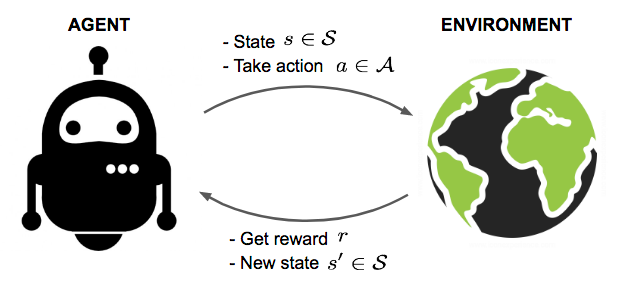
\includegraphics[scale=.24]{Images/RL_illustration.png}
  \caption{Interaction between an Agent and the environment. Image source: \cite{RLsummarylilian}.}
  \label{fig:RL_interaction}
\end{figure}

%------------------------------------------------

\section{Key Concepts of RL}

As we can see in figure \ref{fig:RL_interaction}, the agent interacts with the environment sequentially. Therefore, on time step $t \in \{1,...,T\}$, the agent observe the state of the environment $s_t \in \mathcal{S}$, acts in consequence executing the action $a_t \in \mathcal{A}$, receive its reward $r_t \in \mathcal{R}$ from the environment and observes the new state $s_{t+1} \in \mathcal{S}$.
The tuple $(s_t, a_t, r_t, s_{t+1})$ is known as \emph{transition} step.
This interactions continues until the agent: \textit{i}) Completes the task successfully; \textit{ii}) Fails; \textit{iii}) Reach a time limit. This chain of transition steps from the beginning ($t=1$) until the end ($t=T$) is call \emph{Episode}.
We are interested in environments for which the model that defines them is unknown (\emph{Model-free RL}), and has to be learned explicitly as part of the algorithm (otherwise the optimal solution can be found by means of \emph{Dynamec Programming} (DP)).

\noindent This interaction  is an example of a Markov Decision Process (MDP)\cite{Sutton1998} $\mathcal{M}=<\mathcal{S}, \mathcal{A}, P, R>$, where:

\begin{itemize}
    \item $\mathcal{S}$ is the set of states that holds the Markov property\footnote{The conditional probability distribution of future states (conditional on both past and present states) depends only upon the present state, not on the sequence of events that preceded it, i.e. $P(s_{t+1}|s_{t}, s_{t-1},\dots, s_1)=P(s_{t+1}|s_{t})$.}.
    \item $\mathcal{A}$ is the set of actions.
    \item $P$ is the transition probability function: $P(s_{t+1},r_{t+1}|s_t, a_t)$.
    \item $R$ is the reward function: $R(s_t, a_t):=\mathbb{E}[R_{t+1}|s_t,a_t]=\sum_{r\in \mathcal{R}}r \sum_{s' \in \mathcal{S}}P(s',r|s_t, a_t)$.
\end{itemize}

However, note that in fact we are not interested in maximizing the reward on each time step but the \emph{Return} instead, which is the future cumulative reward\footnote{This might sound counterintuitive. However, think of it as when you have to make less rewarding decisions in the short term (e.g. watching Netflix instead of studying) in order to achieve a greater long-term goal (e.g. approving an exam).}:
\begin{equation}
  G_t := \sum_{k=0}^T \gamma^k r_{t+k+1}
\end{equation}
where $\gamma \in [0,1]$ is the discount factor meant to encourage the agent to finish the task as soon as possible, since in practice time is a valuable resource.

Recall that the ultimate goal of RL is to find an optimal strategy, such that it maximize the Return. Then, how to choose actions that help us to achieve this? The answer is the \emph{Policy} $\pi$. The policy is the functions that defines the agent’s behavior and maps a state $s$ to an action $a$. This function can be either deterministic or stochastic:

\begin{itemize}
  \item \textbf{Deterministic}: $\pi: \mathcal{S} \rightarrow \mathcal{A}$; i.e. $\pi(s)=a$.
  \item \textbf{Stochastic}: $\pi: \mathcal{S} \times \mathcal{A} \rightarrow [0, 1]$; i.e. $\pi(a|s)=P_{\pi}(A=a|S=s)$.
\end{itemize}

Now that we have (more or less) a clear idea of what RL seeks (maximize the return $G$) and how to do it (by finding an optimal policy $\pi$), we need to define a way to quantify how good a state $s$ is (in terms of the return $G$) in a given environment (when we follow a policy $\pi$), and how good an action $a$ is (in terms of the return $G$) when the environment is in state $s$ (and when we follow a policy $\pi$). This is done through the \emph{State-value} and \emph{Action-value} functions respectively:
\begin{itemize}
    \item \textbf{State-value}: $V_{\pi}(s):= \mathbb{E}_{\pi}[G_t|s_t=s]$.
    \item \textbf{Action-value}: $Q_{\pi}(s, a):= \mathbb{E}_{\pi}[G_t|s_t=s, a_t=a]$.
\end{itemize}

%-------------------------------------------------------------------------------

\section{Policy Gradient methods}

There are several ways to approximate an optimal strategy. For example, in \emph{action-value} methods we learn the values of actions and then select
actions based on their estimated action values (e.g. \textit{Q-learning}). Nevertheless, this means that their policies would not even exist without the action-value estimates \cite{Sutton1998}.

However, in \emph{Policy Gradient} we consider methods that instead learn a parameterized policy (e.g. an artificial neural network) that can select actions without consulting a value function\footnote{A value function may still be used to learn the policy parameter, but is not required for action selection.}.
Therefore, we write
$$\pi(a|s,\boldsymbol{\theta}) = Pr(A_t=a | S_t=s; \boldsymbol{\theta}_t=\boldsymbol{\theta})$$
 to denote the probability that the action $a$ is taken, given the parameters $\boldsymbol{\theta}$ and that the environment is in state $s$ at time $t$.
Then, we can approximate an optimal policy by means of gradient ascent while maximizing a performance measure $J(\boldsymbol{\theta})$:

\begin{equation}
  \boldsymbol{\theta}_{t+1} = \boldsymbol{\theta}_{t} + \widehat{\alpha \nabla J(\boldsymbol{\theta}_t)}
  \label{eq:learn_rule}
\end{equation}

\noindent where $\widehat{\nabla J(\boldsymbol{\theta})}$ is a stochastic unbiased estimator of $\nabla J(\boldsymbol{\theta})$ (i.e. $\mathbb{E}[\widehat{\nabla J(\boldsymbol{\theta})}] = \nabla J(\boldsymbol{\theta})$).

Then, how to define the performance measure $J(\boldsymbol{\theta})$?
There are many ways to define $J$, which depend mainly on the method used to approximate the policy.
However, since we are considering only episodic environments\footnote{The definition and explanation of the continuous case is out of the scope of this work.}, then we seek to maximize the return in a given time step ($G_t$), and therefore we define it as the value of the state $s_t$ , i.e. $J(\boldsymbol{\theta}):=V_{\pi_{\boldsymbol{\theta}}}(s_t)$.

Since we are approximating an optimal policy, we need to express $\nabla J(\boldsymbol{\theta})$ in terms of $\pi(\boldsymbol{\theta})$. Therefore, after marginalize $V_{\pi_{\boldsymbol{\theta}}}(s_t)$ over the action space $\mathcal{A}$ and applying Baye's rule we have:

\begin{equation}
  \begin{split}
    \nabla J({\boldsymbol{\theta}}) &= \nabla V_{\pi_{\boldsymbol{\theta}}}(s_t)\\
    &= \nabla \sum_{a_t \in \mathcal{A}} \pi (a_t|s_t; \boldsymbol{\theta}) Q_{\pi_{\boldsymbol{\theta}}}(s_t,a_t)
  \end{split}
  \label{eq:grad}
\end{equation}

The problem is that the right hand side of equation \ref{eq:grad} depends on both the action selections and the distribution of states in which those selections are made, and that both of these are affected by the policy parameter. Fortunately, with the aid of the \emph{Policy Gradient Theorem} we can reformulate $\nabla J({\boldsymbol{\theta}})$ to be proportional to $\nabla \pi (a_t|s_t; \boldsymbol{\theta})$\footnote{A complete proof to this result can be found in page 325 of \cite{Sutton1998}.}:

\begin{equation*}
\resizebox{.95\linewidth}{!}{%
  $\begin{split}
    \nabla J({\boldsymbol{\theta}}) &\propto
    \sum_{s_t \in \mathcal{S}} \mu (s_t) \sum_{a_t \in \mathcal{A}} Q_{\pi_{\boldsymbol{\theta}}}(s_t,a_t) \nabla \pi (a_t|s_t; \boldsymbol{\theta}) \\
    &=\sum_{s_t \in \mathcal{S}} \mu (s_t) \sum_{a_t \in \mathcal{A}} \pi (a_t|s_t; \boldsymbol{\theta}) Q_{\pi_{\boldsymbol{\theta}}}(s_t,a_t) \frac{\nabla \pi (a_t|s_t; \boldsymbol{\theta})}{\pi (a_t|s_t; \boldsymbol{\theta})} \\
    &=\sum_{s_t \in \mathcal{S}} \mu (s_t) \sum_{a_t \in \mathcal{A}} \pi (a_t|s_t; \boldsymbol{\theta}) Q_{\pi_{\boldsymbol{\theta}}}(s_t,a_t) \nabla \log{\pi (a_t|s_t; \boldsymbol{\theta})} \\
    &= \mathbb{E}_{s \sim \mu_{\pi}, a \sim \pi_{\theta}}[Q_{\pi_{\boldsymbol{\theta}}}(S_t,A_t) \nabla \log{\pi (A_t|S_t; \boldsymbol{\theta})}] \\
    &= \mathbb{E}_{s \sim \mu_{\pi}, a \sim \pi_{\theta}}[G_t \nabla \log{\pi (A_t|S_t; \boldsymbol{\theta})}] \\
  \end{split}
  $}
\end{equation*}


\noindent where $\mathbb{E}_{s \sim \mu_{\pi}, a \sim \pi_{\theta}}$ is the expectation of both state and action distributions following the policy $\pi_{\boldsymbol{\theta}}$; $A_t$ and $S_t$ are random variables ($A_t \sim \mu_{\pi}$ and $S_t \sim \pi_{\theta}$); and $Q_{\pi_{\boldsymbol{\theta}}}(S_t,A_t)$ can be replaced by $G_t$ since $\mathbb{E}[G_t| S_t,A_t] = Q_{\pi_{\boldsymbol{\theta}}}(S_t,A_t)$.

Therefore, our learning rule defined in \ref{eq:learn_rule} can be updated to:

\begin{equation*}
  \boldsymbol{\theta}_{t+1} = \boldsymbol{\theta}_{t} + \alpha G_t \nabla \log{\pi (A_t|S_t; \boldsymbol{\theta})}
\end{equation*}

However, the \emph{Policy Gradient Theorem} can be generalized to include a comparison of the action-value function to an arbitrary baseline $b(s)$ \cite{Sutton1998}, which can be any function, even a random variable, as long as it does not depend on the action $a$:

\begin{equation*}
  \nabla J({\boldsymbol{\theta}}) \propto
  \sum_{s_t \in \mathcal{S}} \mu (s_t) \sum_{a_t \in \mathcal{A}} \left( Q_{\pi_{\boldsymbol{\theta}}}(s_t,a_t) - b(s_t) \right) \nabla \pi (a_t|s_t; \boldsymbol{\theta})
\end{equation*}

the last equation remains valid because the subtracted quantity is zero:

\begin{equation*}
  \begin{split}
    \sum_{a_t \in \mathcal{A}} b(s_t) \nabla \pi (a_t|s_t; \boldsymbol{\theta}) &=
    b(s_t) \sum_{a_t \in \mathcal{A}} \nabla \pi (a_t|s_t; \boldsymbol{\theta})\\
    &= b(s_t) \nabla 1 \\
    &= 0
  \end{split}
\end{equation*}

Finally, we can use this to derive a new update rule that includes a general baseline:

\begin{equation}
  \boldsymbol{\theta}_{t+1} = \boldsymbol{\theta}_{t} + \alpha (G_t - b(S_t)) \nabla \log{\pi (A_t|S_t; \boldsymbol{\theta})}
  \label{eq:learn_rule_bl}
\end{equation}

%-------------------------------------------------------------------------------

\section{Actor-Critic}

Equation \ref{eq:learn_rule_bl} give us a rule to update the policy parameters $\boldsymbol{\theta}$ on every time step. However, this rule is incomplete since we don't know the value of the return $G_t$. But, what if we express $G_t$ in something that depends on the state, so we can learn it in parallel with the policy $\pi_{\boldsymbol{\theta}}$? Fortunately, $G_t \approx V_{\pi}(s_t)$ (since recall that $V_{\pi}(s):= \mathbb{E}_{\pi}[G_t|s_t=s]$).

However, if we just replace $G_t$ by a parameterized approximation of the state-value function (e.g. $V(s;\boldsymbol{w})$), we would not be using the feedback (reward) given by the environment, and hence we would hardly learn something meaningful. Instead, we could use the identity $G_t = R_{t+1} + \gamma G_{t+1}$ and replace $G_{t+1}$ with $V(S_{t+1};\boldsymbol{w})$, so we can actually use the observed reward $R_{t+1}$ on every time step. Hence, the update rule ends as:

\begin{equation}
  \resizebox{.91\linewidth}{!}{%
  $
    \boldsymbol{\theta}_{t+1} = \boldsymbol{\theta}_{t} + \alpha (R_{t+1} + \gamma V(S_{t+1};\boldsymbol{w}) - b(S_t)) \nabla \log{\pi (A_t|S_t; \boldsymbol{\theta})}
  $
  }
  \label{eq:learn_rule_3}
\end{equation}

Equation \ref{eq:learn_rule_3} shows way this method is call \emph{Actor-Critic}. Actor-critic methods consist of two models, which may optionally share parameters:
\begin{itemize}
  \item \textbf{Critic} updates the parameters $\boldsymbol{w}$ of the state-value\footnote{Depending on the algorithm, the Critic could be instead the action-value $Q(a|s;\boldsymbol{w})$ function.} function $V(s; \boldsymbol{w})$ and measures (criticize) how good the taken action is.
  \item \textbf{Actor} updates the parameters $\boldsymbol{\theta}$ of the policy $\pi(a|s; \boldsymbol{\theta})$ function, in the direction suggested by the critic.
\end{itemize}

Equation \ref{eq:learn_rule_3}, give us a rule that we can finally implement and use. However, there are still one last detail, the definition of the baseline $b(s)$. In general, the baseline leaves the expected value of the update unchanged, but it can significantly reduce the variance (and thus speed the learning). In MDPs the baseline should vary with the state.
In some states all actions may have high values and we would need a high baseline to differentiate the higher valued actions from the less highly valued ones; in other states all actions may have low values and a low baseline would be appropriate.
Therefore, one natural choice for the baseline is an estimate of the state-value function, $V(S_{t};\boldsymbol{w})$ \cite{Sutton1998}.
Hence, the update rule ends as:

\begin{equation*}
  \resizebox{1\linewidth}{!}{%
  $
    \boldsymbol{\theta}_{t+1} = \boldsymbol{\theta}_{t} + \alpha (R_{t+1} + \gamma V(S_{t+1};\boldsymbol{w}) - V(S_{t};\boldsymbol{w})) \nabla \log{\pi (A_t|S_t; \boldsymbol{\theta})}
  $
  }
  %\label{eq:learn_rule_4}
\end{equation*}

But, what about the update rule for the state-value function $V(S;\boldsymbol{w})$ parameters $\boldsymbol{w}$? As we did with the policy, we need to start by defining an objective function $E(\boldsymbol{w})$. Since $V: \mathbb{R} \rightarrow \mathbb{R}$ (regression problem), we can just use the \emph{Squared Error} as a loss function (i.e. $E(\boldsymbol{w}):=(V_{\pi}(S) - V(S;\boldsymbol{w}))^2$), and then optimize the approximator parameters $\boldsymbol{w}$ while minimizing it. Therefore:

\begin{equation*}
  \begin{split}
    \nabla E(\boldsymbol{w}) &= \nabla (V_{\pi}(S_t) - V(S_t;\boldsymbol{w}))^2 \\
    &= 2(V_{\pi}(S_t)) - V(S_t;\boldsymbol{w})) \nabla V(S_t;\boldsymbol{w})) \\
    &\approx 2(R_{t+1} + \gamma V(S_{t+1};\boldsymbol{w}) - V(S_t;\boldsymbol{w})) \nabla V(S_t;\boldsymbol{w}))
  \end{split}
\end{equation*}

Therefore, the update rule for $\boldsymbol{w}$ is:

\begin{equation*}
  \resizebox{1\linewidth}{!}{%
  $
    \boldsymbol{w}_{t+1} = \boldsymbol{w}_t - \alpha (R_{t+1} + \gamma V(S_{t+1}; \boldsymbol{w}) - V(S_{t}; \boldsymbol{w})) \nabla V(S_{t}; \boldsymbol{w})
    $
  }
  %\label{eq:learn_rule_w}
\end{equation*}

A pseudocode for an algorithm which approximate both the policy and the state-value function is shown in \ref{alg:A2C}.

%\resizebox{.95\linewidth}{!}{%
\begin{algorithm}[h]
 \textbf{Input}: differentiable policy and state-value function parameterization $\pi(a|s;\boldsymbol{\theta})$ and $V(s;\boldsymbol{w})$\;
 \textbf{Parameters}: step sizes $\alpha^{\boldsymbol{\theta}}>0,\  \alpha^{\boldsymbol{w}}>0$ and discount factor $\gamma \in [0,1]$\;
 Initialize policy and state-value parameters $\boldsymbol{\theta}\in\mathbb{R}^d$ and $\boldsymbol{w}\in\mathbb{R}^{d'}$\;
 \For{Episode = 1, 2, ...}{
  \While{$S_t$ is not terminal (for each time step $t$)}{
    Sample action $A_t \sim \pi(\cdot|S_t;\boldsymbol{\theta})$ \;
    Take action $A_t$ and observe $S_{t+1}, R_{t+1}$\;
    \If{$S_{t+1}$ is terminal}{
      $V(S_{t+1}; \boldsymbol{w}) = 0$\;
    }
    $\delta \gets R_{t+1} + \gamma V(S_{t+1}; \boldsymbol{w}) - V(S_{t}; \boldsymbol{w})$\;
    $\boldsymbol{w} \gets \boldsymbol{w} - \alpha^{\boldsymbol{w}} \delta \nabla V(S_{t}; \boldsymbol{w})$\;
    $\boldsymbol{\theta} \gets \boldsymbol{\theta} + \alpha^{\boldsymbol{\theta}} \delta \nabla \log{\pi(A_{t}|S_{t}; \boldsymbol{\theta})}$\;
    $S_t \gets S_{t+1}$\;
  }
 }
 \caption{Advantage Actor Critic pseudocode \cite{Sutton1998}.}
 \label{alg:A2C}
\end{algorithm}
%}

The \emph{Advantage Actor Critic} showed in algorithm \ref{alg:A2C} was named after the \emph{Advantage} function $A(S_t, A_t):=R_{t+1} + \gamma V(S_{t+1};\boldsymbol{w}) - V(S_{t};\boldsymbol{w})$, which captures how better an action is compared to the others at a given state\footnote{In some sense, instead of having the critic to learn the state values, we make it learn the Advantage values. In that way, the evaluation of an action is based not only on how good the action is, but also how much better it can be.}.

\section{Trust region-based policy optimization}

The Advantage Actor Critic pseudocode shown in algorithm \ref{alg:A2C} should in principle be able to approximate an optimal policy. However, in practice the training process is often unstable. One reason for this is the policy update. Recall that RL algorithms learn from data generated by the interaction between the environment and the agent (i.e. the policy). Therefore, a strong change in the policy means a strong change in the data distribution. Unlike supervised learning, where the learning and data are typically independent (the learning process can not mess the dataset), in RL the training and the data is strongly related. Therefore, a too aggressive update in the policy could lead to a bad policy which will result in poor data, and therefore in a poor training process.

One way to prevent instability in the training process is by adding regularization to the difference between subsequent policies. This can be achieved using the Kullback–Leibler divergence $D_{KL}$ between the actions distribution of the previous policy $\pi_{\theta_{old}}$ and the new policy $\pi_{\theta}$ (\cite{intro2RL} and \cite{Aclecture}:

\begin{equation*}
    D_{KL}(\pi_{\theta_{old}} || \pi_{\theta}) = \mathbb{E} \left[
    \int \pi(A|S;\boldsymbol{\theta}_{old})
    \log{\frac{\pi(A|S;\boldsymbol{\theta})}{\pi(A|S;\boldsymbol{\theta}_{old})}}\text{d}a
    \right]
\end{equation*}

\noindent If the action space $\mathcal{A}$ is not continuous (i.e. discrete), then we can sum over all the actions instead of integrating.

To consider the difference between subsequent policies in our training, we need to transform our original optimization problem (maximize $J(\boldsymbol{\theta})$) into a constrained optimization problem:

\begin{equation}
  \begin{split}
    \text{maximize} \ \ \ \ \ &J(\boldsymbol{\theta})\\
    \text{s.t.} \ \ \ \ \ &D_{KL}(\pi_{\theta_{old}} || \pi_{\theta}) \leq \eta
  \end{split}
  \label{eq:c_opt}
\end{equation}

\noindent where $\eta > 0$ is the regularization hyperparameter (usually small) which specifies how much do we penalize the difference between subsequent policies.

Finally, we can approximate the constrained optimization problem \ref{eq:c_opt} just by maximizing \cite{Vitay}:

\begin{equation}
  J(\boldsymbol{\theta}) - \eta D_{KL}(\pi_{\theta_{old}} || \pi_{\theta})
\end{equation}


%-------------------------------------------------------------------------------
%	REFERENCE LIST
%-------------------------------------------------------------------------------

\printbibliography

%-------------------------------------------------------------------------------

\end{document}
